
\section*{Общая характеристика работы}

\newcommand{\actuality}{\underline{\textbf{\actualityTXT}}}
\newcommand{\progress}{\underline{\textbf{\progressTXT}}}
\newcommand{\aim}{\underline{{\textbf\aimTXT}}}
\newcommand{\tasks}{\underline{\textbf{\tasksTXT}}}
\newcommand{\novelty}{\underline{\textbf{\noveltyTXT}}}
\newcommand{\influence}{\underline{\textbf{\influenceTXT}}}
\newcommand{\methods}{\underline{\textbf{\methodsTXT}}}
\newcommand{\defpositions}{\underline{\textbf{\defpositionsTXT}}}
\newcommand{\reliability}{\underline{\textbf{\reliabilityTXT}}}
\newcommand{\probation}{\underline{\textbf{\probationTXT}}}
\newcommand{\contribution}{\underline{\textbf{\contributionTXT}}}
\newcommand{\publications}{\underline{\textbf{\publicationsTXT}}}


{\actuality} Круг задач, решаемых на высокопризводительных вычислительных системах, очень обширен. Он включает в себя множество исследовательских, оборонных и промышленных задач, в частности моделирование астрофизических процессов и физических процессов в плазменных установках, моделирование поведения вещества при сверхвысоких температурах и давлениях, разработка новых материалов, расчеты аэродинамики первспективных самолетов и автомобилей, преджсказание погоды и задачи биоинформатики.

Все эти очень различные задачи объединяет одно: они предъявляют очень высокие требования к оборудованию и системному программному обеспечению вычислительной системы (ВС). При этом одни задачи  отличаются повышенными требованиями апежде всего к скорости вычислений, другие к быстродействию сетевого оборудования, третьи  к скорости работы файловой системы. Таким образом, возникает вопрос об о расчете быстродействия ВС, отдельной ее подсистемы, или в комплексе, и об определении степени пригодности данной ВС для решения того или иного типа задач. 

Это означает необходимость создания специализированных программ-тестов для определения быстродействия конкретной ВС. В настоящее время существует большое количество подобных программ: Linpack, HPCG, NAS parallel benchmark, SPEChpc96.
Все это многообразие показывает что задача создания теста производительности ВС остается актуальной.


Желательно, чтобы тесты создавались на базе программ, используемых для решения реальных задач для того, чтобы результатом работы теста были бы не только числовые показатели, но и конкретное подтвержение способности тестируемой ВС решать сложные задачи, актуальные с научной или производственной точки зрения. Так, тест Lapack создан на основе методов решения системы линейных уравнений с помощью LU-факторизации, тест HPCG - на основе метода сопряженных градиентов, NAS parallel benchmark ориентирован на задачи гидро и газодинамики.



Кроме тестирования скорости выполнения арифметических операций очень важное значение имеет произвоительность системы ввода-вывода. Это проблема, имеющая самостоятельное научное значение. о чем свидетельствует, в частности, доклад  <<Do you know what your I/O is doing>>. В приложении к конкретным задачам математического моделирования время собственно решения задачи на высокопроизводительной ВС иногда оказывается меньше, чем время записи результатов на жесткие диски.
Таким образом анализ производительность системы ввода-вывода должен быть включен в тест производительности.
Одним из немногих тестовых пакетов, решающих эту задачу, является Intel Cluster Checker - набор программ, производящий всестороннее тестирование кластерной системы, и каждой отдельной подсистемы, и вопросы совместного функционирования подсистем. 

Для сокращения временных и ресурсных затрат на проведение тестирования необходимо создавать тесты на базе программ, реализующих такие математические методы, которые предъявляют высокие требования сразу к нескольким, в идеале - ко всем подсистемам тестируемой ВС. 

Одним из таких методов является метод частиц в ячейках.Его достоинством является, с одной стороны, использование в качестве инструментов нескольких существенно различных вычислительных методов, что позволяет исходя из тестированияна методе частиц в ячейках достоверно прогнозировать производительность данной ВС на многих других задачах. С другой стороны, достоинством метода частиук как теста является трудность его эффективной реализации на высокопроизводительных ВС, в частности нерегулярный доступ к памяти, недетерминированный объем и частнота межпроцессорных пересылок и очень больший объем выдач - проблемы с которыми е всегда и не в полном обеме удается справлятся на уровне прикладного ПО. Фактическая эффективность работы ВС с таким сложным приложением является хорошей характеристикой качества оборудования и системного ПО.

Таким образом, \textbf{актуальность работы} заключается в необходимости создания именно комплексного теста производительнсти вычислительных систем, охватывающего все аспекты, влияющие на быстродействие: процессорные элементы, шину памяти, модули памяти, параллельную файловую систему, жесткие диски, позволяющего определить  реальную скорость счета с учетом того, что данные находятся не в регистрах процессора и должны быть туда загружены таким образом выяснить реальное быстродействие системы на широком спектре задач математического моделирования на высокопроизводительных вычислительных системах. 

% {\progress} 
% Этот раздел должен быть отдельным структурным элементом по
% ГОСТ, но он, как правило, включается в описание актуальности
% темы. Нужен он отдельным структурынм элемементом или нет ---
% смотрите другие диссертации вашего совета, скорее всего не нужен.

{\aim} данной работы является 

 разработка методики и создание реализующей ее программы для комплекспой оценки производительности ВС с учетом функционирования всех подсистем  и выявления скорости решения реальных задач. Таким образом предполагается представить альтернативу традиционной методике оценки производительности ВВС, основанной только лишь на количестве операций в секунду.  


Для~достижения поставленной цели необходимо было решить следующие {\tasks}:
\begin{enumerate}
  \item Исследовать, разработать, вычислить и~т.\:д. и~т.\:п.
  \item Исследовать, разработать, вычислить и~т.\:д. и~т.\:п.
  \item Исследовать, разработать, вычислить и~т.\:д. и~т.\:п.
  \item Исследовать, разработать, вычислить и~т.\:д. и~т.\:п.
\end{enumerate}


{\novelty}
\begin{enumerate}
  \item Впервые \ldots
  \item Впервые \ldots
  \item Было выполнено оригинальное исследование \ldots
\end{enumerate}

{\influence} \ldots

{\methods} \ldots

{\defpositions}
\begin{enumerate}
  \item Первое положение
  \item Второе положение
  \item Третье положение
  \item Четвертое положение
\end{enumerate}
В папке Documents можно ознакомиться в решением совета из Томского ГУ
в~файле \verb+Def_positions.pdf+, где обоснованно даются рекомендации
по~формулировкам защищаемых положений. 

{\reliability} полученных результатов обеспечивается \ldots \ Результаты находятся в соответствии с результатами, полученными другими авторами.


{\probation}
Основные результаты работы докладывались~на:
перечисление основных конференций, симпозиумов и~т.\:п.

{\contribution} Автор принимал активное участие \ldots

%\publications\ Основные результаты по теме диссертации изложены в ХХ печатных изданиях~\cite{Sokolov,Gaidaenko,Lermontov,Management},
%Х из которых изданы в журналах, рекомендованных ВАК~\cite{Sokolov,Gaidaenko}, 
%ХХ --- в тезисах докладов~\cite{Lermontov,Management}.

\ifnumequal{\value{bibliosel}}{0}{% Встроенная реализация с загрузкой файла через движок bibtex8
    \publications\ Основные результаты по теме диссертации изложены в XX печатных изданиях, 
    X из которых изданы в журналах, рекомендованных ВАК, 
    X "--- в тезисах докладов.%
}{% Реализация пакетом biblatex через движок biber
%Сделана отдельная секция, чтобы не отображались в списке цитированных материалов
    \begin{refsection}[vak,papers,conf]% Подсчет и нумерация авторских работ. Засчитываются только те, которые были прописаны внутри \nocite{}.
        %Чтобы сменить порядок разделов в сгрупированном списке литературы необходимо перетасовать следующие три строчки, а также команды в разделе \newcommand*{\insertbiblioauthorgrouped} в файле biblio/biblatex.tex
        \printbibliography[heading=countauthorvak, env=countauthorvak, keyword=biblioauthorvak, section=1]%
        \printbibliography[heading=countauthorconf, env=countauthorconf, keyword=biblioauthorconf, section=1]%
        \printbibliography[heading=countauthornotvak, env=countauthornotvak, keyword=biblioauthornotvak, section=1]%
        \printbibliography[heading=countauthor, env=countauthor, keyword=biblioauthor, section=1]%
        \nocite{%Порядок перечисления в этом блоке определяет порядок вывода в списке публикаций автора
                vakbib1,vakbib2,%
                confbib1,confbib2,%
                bib1,bib2,%
        }%
        \publications\ Основные результаты по теме диссертации изложены в~\arabic{citeauthor}~печатных изданиях, 
        \arabic{citeauthorvak} из которых изданы в журналах, рекомендованных ВАК, 
        \arabic{citeauthorconf} "--- в~тезисах докладов.
    \end{refsection}
    \begin{refsection}[vak,papers,conf]%Блок, позволяющий отобрать из всех работ автора наиболее значимые, и только их вывести в автореферате, но считать в блоке выше общее число работ
        \printbibliography[heading=countauthorvak, env=countauthorvak, keyword=biblioauthorvak, section=2]%
        \printbibliography[heading=countauthornotvak, env=countauthornotvak, keyword=biblioauthornotvak, section=2]%
        \printbibliography[heading=countauthorconf, env=countauthorconf, keyword=biblioauthorconf, section=2]%
        \printbibliography[heading=countauthor, env=countauthor, keyword=biblioauthor, section=2]%
        \nocite{vakbib2}%vak
        \nocite{bib1}%notvak
        \nocite{confbib1}%conf
    \end{refsection}
}
При использовании пакета \verb!biblatex! для автоматического подсчёта
количества публикаций автора по теме диссертации, необходимо
их~здесь перечислить с использованием команды \verb!\nocite!.
 % Характеристика работы по структуре во введении и в автореферате не отличается (ГОСТ Р 7.0.11, пункты 5.3.1 и 9.2.1), потому её загружаем из одного и того же внешнего файла, предварительно задав форму выделения некоторым параметрам

%Диссертационная работа была выполнена при поддержке грантов ...

\underline{\textbf{Объем и структура работы.}} Диссертация состоит из~введения,
пяти глав, заключения и~приложения. Полный объем диссертации
\textbf{ХХХ}~страниц текста с~\textbf{ХХ}~рисунками и~5~таблицами. Список литературы содержит \textbf{ХХX}~наименование.

\section*{Содержание работы}
Во \underline{\textbf{введении}} 
обоснована актуальность темы исследования и степень
ее разработанности, сформулированы цели и задачи работы, показана ее научная новизна, теоретическая и практическая значимость; представлены положения, выносимые на защиту, а также степень достоверности и апробация результатов.






\underline{\textbf{Первая глава}} посвящена описанию созданной в рамках диссертационной работы реализация метода частиц в ячейках на параллельных ВС с использованием различных типов ускорителей вычислений. 

\underline{\textbf{Вторая глава}} содержит проведенный обзор литературы по вычислениям, проводимых на современных петафлопсных и перспективных экзафлопсных ВС. В частности выявлены вычислительные алгоритмы, которым уделяется особенное внимание применительно к вычислениям на таких ВС.
В обзорную часть данной диссертационной работы вошло 298 статей за период с 2010 по 2016 год в следующих журналах:Future Generation Computer Systems, Procedia Computers Science, Journal of Parallel and Distributed Computing, Parallel Computing, Journal of Computational Physics, Computer Physics Communications и др.  Распределение статей по приложениям показано в таблице \ref{tab_physics}.

\begin{table}[ht]
	\caption{Распределение по приложениям статей относящихся к тематике <<экзафлопсные вычисления>>}
	\begin{center}
		\begin{tabular}{|c|c|}
			\hline
			вычислительная гидродинамика & 27  \\ \hline 
			ядерные технологии & 17       \\ \hline  
			физика плазмы & 11  \\ \hline 
			разработка новых материалов & 10  \\ \hline 
			предсказание погоды & 10 \\ \hline 
			биомедицинские приложения & 9 \\ \hline 
			астрофизика и космология & 6  \\ \hline 
			молекулярная динамика   & 6   \\ \hline 
			мультифизика & 6              \\ \hline 
			геофизика & 6  \\ \hline 
			финансы & 2  \\ \hline 
		\end{tabular}
	\end{center}
	\label{tab_physics}
\end{table}
Комплексный тест производительности высокопроизводительных ВС должен включать в себя алгоритмы, аналогичные используемым в перечисленных приложениях по создаваемой нагрузке на ВС. Можно показать что метод частиц в ячейках соотвествует этому требованию и таким образом на основании проведенных расчетов по методу частиц в ячейках можно с высокой достоверностью предсказывать эффективность работы ВС на приложениях из приведенного списка. Ограничимся тремя наиболее актуальными (т.е. с наибольшим числом статей приложениями из приведенного списка) и пропуская физику плазмы:
\begin{itemize}
	\item \textbf{Вычислительная гидродинамика:} большая часть численных методов использует вычисления на сетке с регулярным доступом к памяти. Это означает, что нагрузка на процессорные элементы и оперативную память аналогична вычислению электромагнитных полей в методе частиц в ячейках
	\item \textbf{Ядерные технологии}: под этим название в обзоре фигурирует моделирование различных процессов, протекающих в ядерных реакторах выполняемое преимущественно на основе метода Монте-Карло, который является близким аналогом метода частиц в ячейках, с той разницей что для его работы требуется меньшее количество синхронизаций между параллельными процессами
	\item \textbf{Разработка новых материалов}: это квантовохимические расчеты структуры и поведения молекул, вычисление супер-многомерных интегралов в различных приближениях. Нагрузка создаваемая данными методами на ВС может достоверно эмулироваться соответвенно этапом расчета движения частиц и этапом вычисления электромагнитного поля в методе частиц в ячейках.
\end{itemize}	    	
Обобщая, можно сказать, что поскольку метод частиц в ячейках содержит участки кода с высокой вычислительной интенсивностью и с низкой, вычислительные процедуры с регулярным доступом к памяти и с нерегулярным, при использовании кэша разных уровней и без такового, а также параллельные коммуникации всех видов, то с использованием результатов тестирования ВС на методе частиц в ячейках можно предсказать эффективность реализации на данной ВС любого из существующих параллельных вычислительных методов и использующего этот метод физического приложения.

В \underline{\textbf{третьей главе}} описана методика измерения характеристик ВС с помощью программы, релизующей метод частиц в ячейках. 

Предложена методика комплексной оценки тестируемой ВС с точки зрения возможности эффективной реализзации математических моделей на основе определения баланса между скоростью счета и скоростью пересылки данных между узлами ВС. Баланс определяется на основе усреднения данных расчетов по методу частиц в ячейках, который используется в качестве оценки снизу по скорости счета и оценки сверху по памяти для большинства существующих математических методов.

Кроме того, на основе проведенных расчетов измерена скорость счета и скорость перемещения данных для нескольких протестированных ВС.   

\textbf{Расчет производительности процессорных элементов}

Для того, чтобы отделить время счета от времени обращения к оперативной памяти было рассмотрено время работы процедуры,
реализующей одномерное преобразование Фурье, которая является частью физической диагностики, используемой в при моделировании динамики плазмы. Измереннное время с учетом известного размера данных и и количества операций в БПФ (\textit{Е.П.Овсянников и др.}), переводится во флопсы. Сравнительная производительность процессорных элементов некоторых из рассмотренных в диссертационной работе ВС выглядит как показано на рисунке  \ref{procs_flops}:

\begin{figure}[htb]
	\begin{center}
		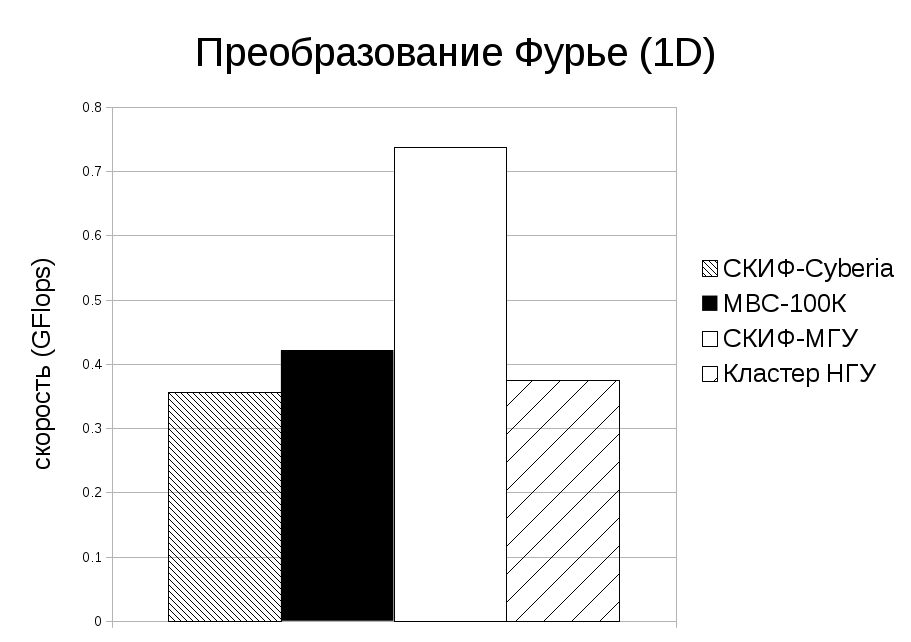
\includegraphics[height=7cm,keepaspectratio]{auto_pics/processor_FLOPS.png}
	\end{center}
	\caption{Производительность процессоров Intel Xeon, измеренная в ходе выполнения одномерного преобразования Фурье на некоторых кластерах. Размерность преобразования $N=64$. Измерения выполнены в 2010 г.}
	\label{procs_flops}
\end{figure} 


\underline{\textbf{Четвертая глава}} посвящена 
\underline{\textbf{Пятая глава}} посвящена 


Можно сослаться на свои работы в автореферате. Для этого в файле
\verb!Synopsis/setup.tex! необходимо присвоить положительное значение
счётчику \verb!\setcounter{usefootcite}{1}!. В таком случае ссылки на
работы других авторов будут подстрочными.
\ifnumgreater{\value{usefootcite}}{0}{
Изложенные в третьей главе результаты опубликованы в~\cite{vakbib1, vakbib2}.
}{}
Использование подстрочных ссылок внутри таблиц может вызывать проблемы.

В \underline{\textbf{четвертой главе}} приведено описание 

В \underline{\textbf{заключении}} приведены основные результаты работы, которые заключаются в следующем:
%% Согласно ГОСТ Р 7.0.11-2011:
%% 5.3.3 В заключении диссертации излагают итоги выполненного исследования, рекомендации, перспективы дальнейшей разработки темы.
%% 9.2.3 В заключении автореферата диссертации излагают итоги данного исследования, рекомендации и перспективы дальнейшей разработки темы.
%\begin{enumerate}
 В работе предложена и реализована оригинальная методика комплексного тестирования мультиархитектурных параллельных вычислительных систем, основанная на используемой в реальных расчетах программе для математического моделирования. а именно на реализации метода частиц в ячейках.
 
 Особенностями предложенной методики комплексного тестирования являются возможность определения для конкретной ВС абсолютной оценки, основанной на степени пригодности данной ВС для решения задач математического моделирования, метод измерения возрастания потока данных в коммуникационной сети ВС, а также оценка эффективности реализации вычислительных алгоритмов для мультиархитектурных ВС.
 
 \textbf{Рекомендации и перспективы дальнейшей разработки темы.}
 Основным направлением совершенствования разработанного теста является автоматическая выработка рекомедаций по оптимизации кода, охватывающих не только методом частиц в ячейках но и остальные наиболее часто используемые в математическом моделировании методы,  под конкретную протестированную ВС.
 
 Одним из наиболее важных вариантов дальнейшего развития программы-теста, созданного в диссертационной работе является перенос на не охваченные в текущем варианте платформы, такие как Android, процессоры архитектуры Sunway.
 
 Кроме того, необходимостью является апробация теста на крупных высокопроизводительных ВС мощностью более петафлопса, а также - возможно, после специальной адаптации схемы расчета движения частиц - на ВС векторной архитектуры.
 
 
 
 
 
  
 
 
%\end{enumerate}




\ifdefmacro{\microtypesetup}{\microtypesetup{protrusion=false}}{} % не рекомендуется применять пакет микротипографики к автоматически генерируемому списку литературы
\ifnumequal{\value{bibliosel}}{0}{% Встроенная реализация с загрузкой файла через движок bibtex8
  \renewcommand{\bibname}{\large \authorbibtitle}
  \nocite{*}
  \insertbiblioauthor           % Подключаем Bib-базы
  %\insertbiblioother   % !!! bibtex не умеет работать с несколькими библиографиями !!!
}{% Реализация пакетом biblatex через движок biber
  \ifnumgreater{\value{usefootcite}}{0}{
%  \nocite{*} % Невидимая цитата всех работ, позволит вывести все работы автора
  \insertbiblioauthorcited      % Вывод процитированных в автореферате работ автора
  }{
  \insertbiblioauthor           % Вывод всех работ автора
%  \insertbiblioauthorgrouped    % Вывод всех работ автора, сгруппированных по источникам
%  \insertbiblioauthorimportant  % Вывод наиболее значимых работ автора (определяется в файле characteristic во второй section)
  \insertbiblioother            % Вывод списка литературы, на которую ссылались в тексте автореферата
  }
}
\ifdefmacro{\microtypesetup}{\microtypesetup{protrusion=true}}{}
